Presentamos los doce tipos de orden para los cuales existe una descomposición en thrackles máximos.
\begin{figure}[h]
    \centering
    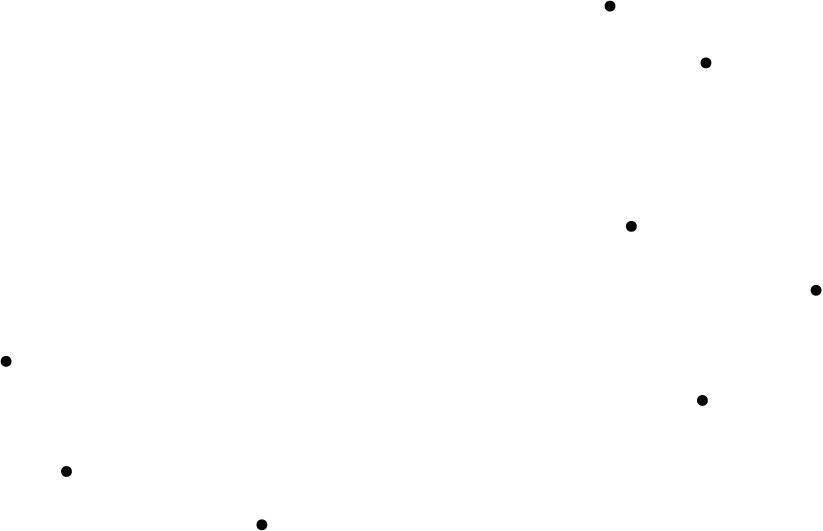
\includegraphics[width=0.8\linewidth, frame]{8_12.png}
    \caption{Tipo de orden número 12 para $n=8$}
\end{figure}
\begin{figure}
    \centering
    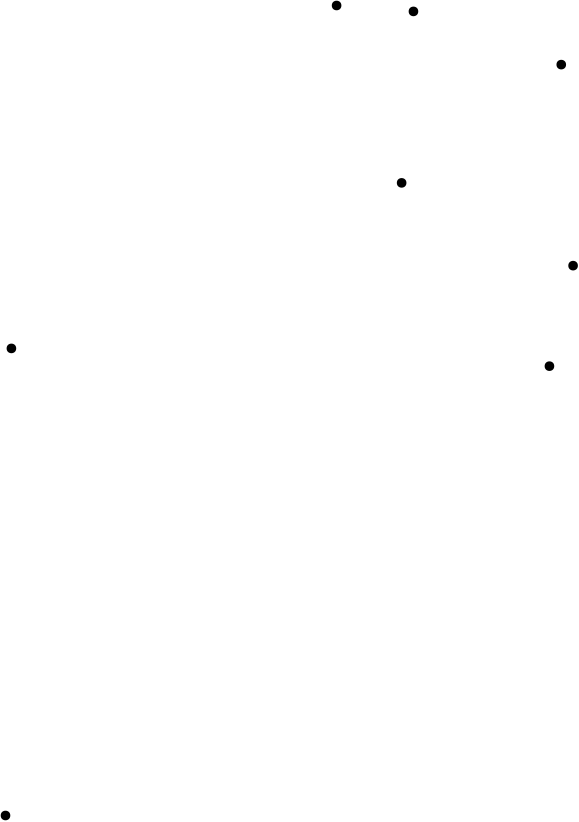
\includegraphics[width=0.8\linewidth, frame]{8_54.png}
    \caption{Tipo de orden número 54 para $n=8$}
\end{figure}
\begin{figure}
    \centering
    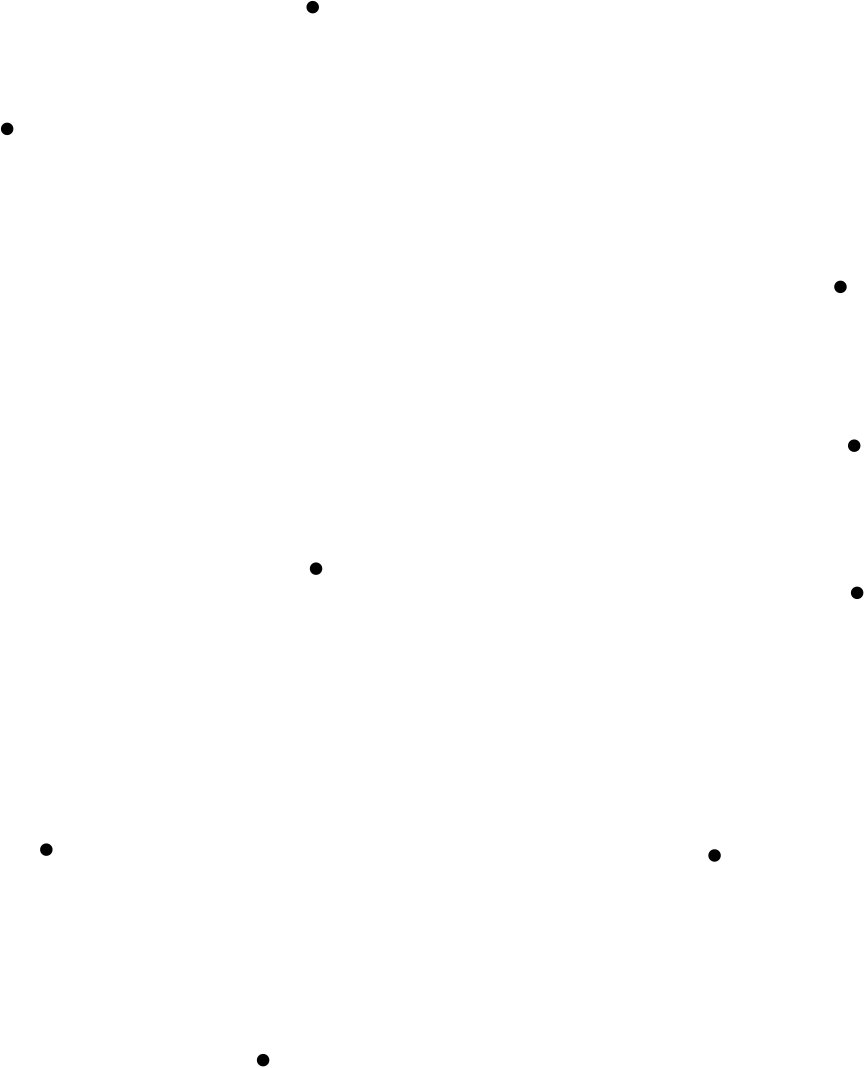
\includegraphics[width=0.8\linewidth, frame]{9_12.png}
    \caption{Tipo de orden número 12 para $n=9$}
\end{figure}
\begin{figure}
    \centering
    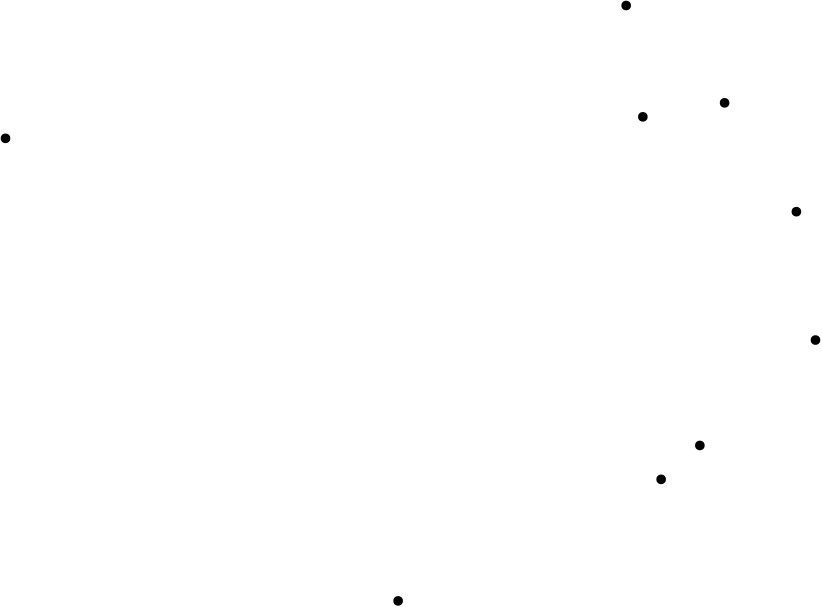
\includegraphics[width=0.9\linewidth, frame]{9_52.png}
    \caption{Tipo de orden número 52 para $n=9$}
\end{figure}
\begin{figure}
    \centering
    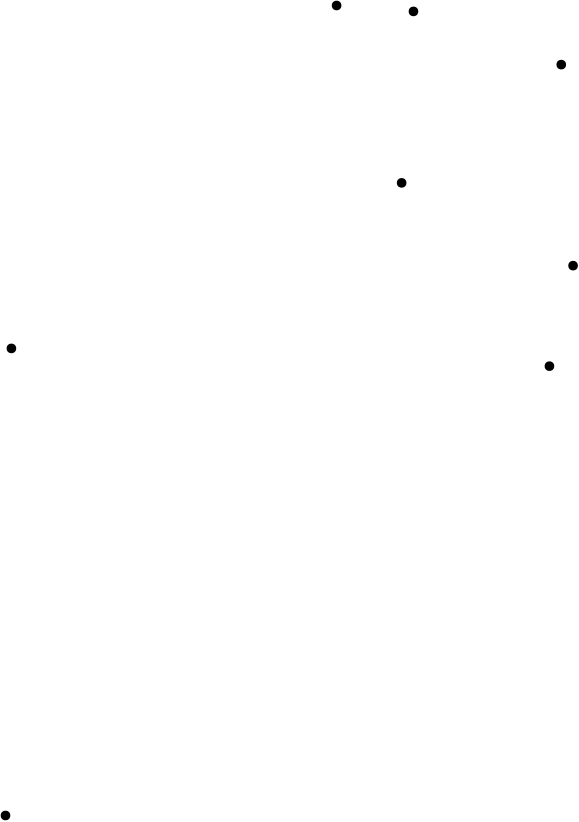
\includegraphics[width=0.9\linewidth, frame]{9_54.png}
    \caption{Tipo de orden número 54 para $n=9$}
\end{figure}
\begin{figure}
    \centering
    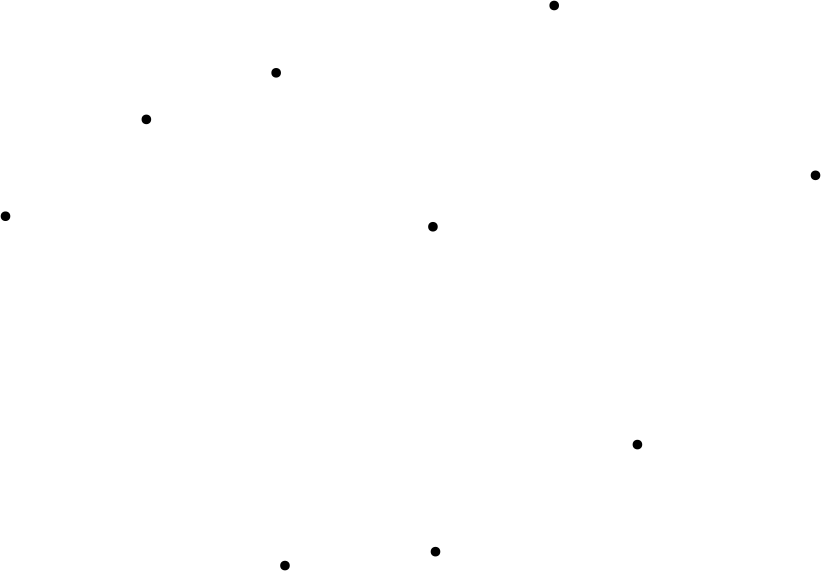
\includegraphics[width=0.9\linewidth, frame]{9_80.png}
    \caption{Tipo de orden número 80 para $n=9$}
\end{figure}
\begin{figure}
    \centering
    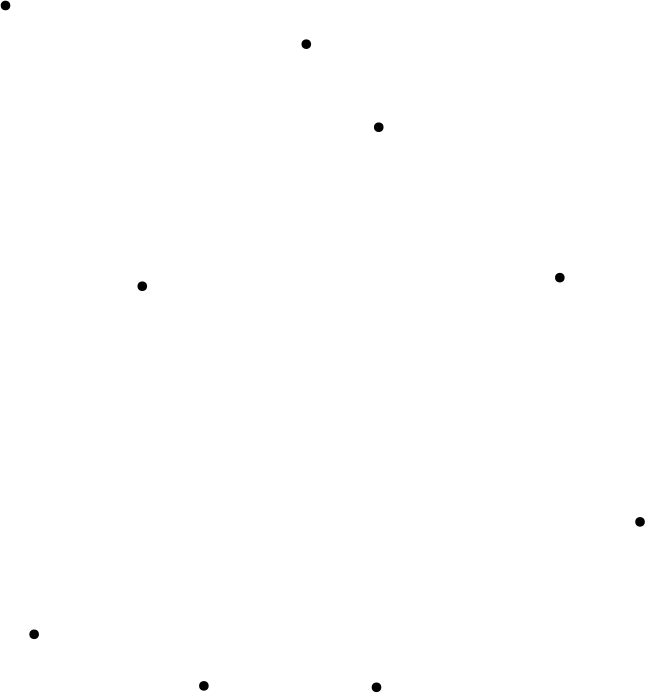
\includegraphics[width=0.9\linewidth, frame]{9_696.png}
    \caption{Tipo de orden número 696 para $n=9$}
\end{figure}

\begin{figure}
    \centering
    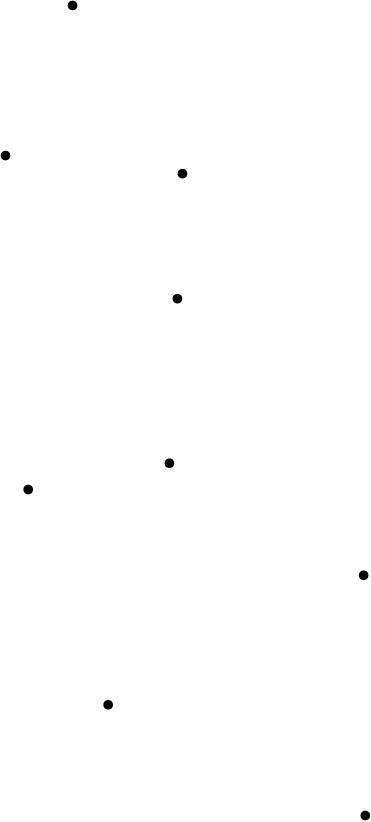
\includegraphics[width=0.6\linewidth, frame]{9_1080.png}
    \caption{Tipo de orden número 1080 para $n=9$}
\end{figure}
\begin{figure}
    \centering
    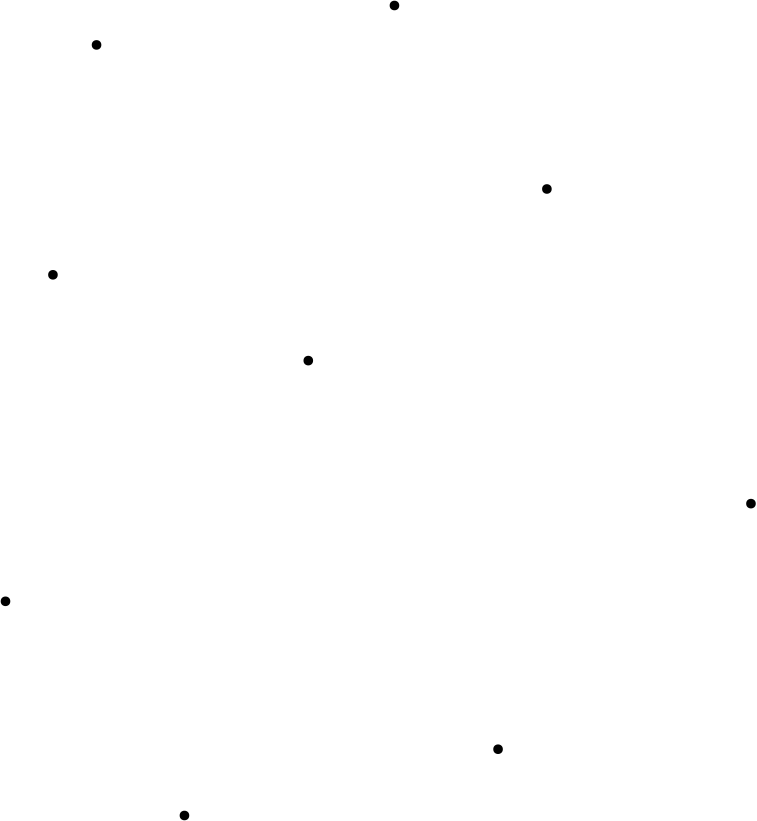
\includegraphics[width=0.9\linewidth, frame]{9_1287.png}
    \caption{Tipo de orden número 1287 para $n=9$}
\end{figure}
\begin{figure}
    \centering
    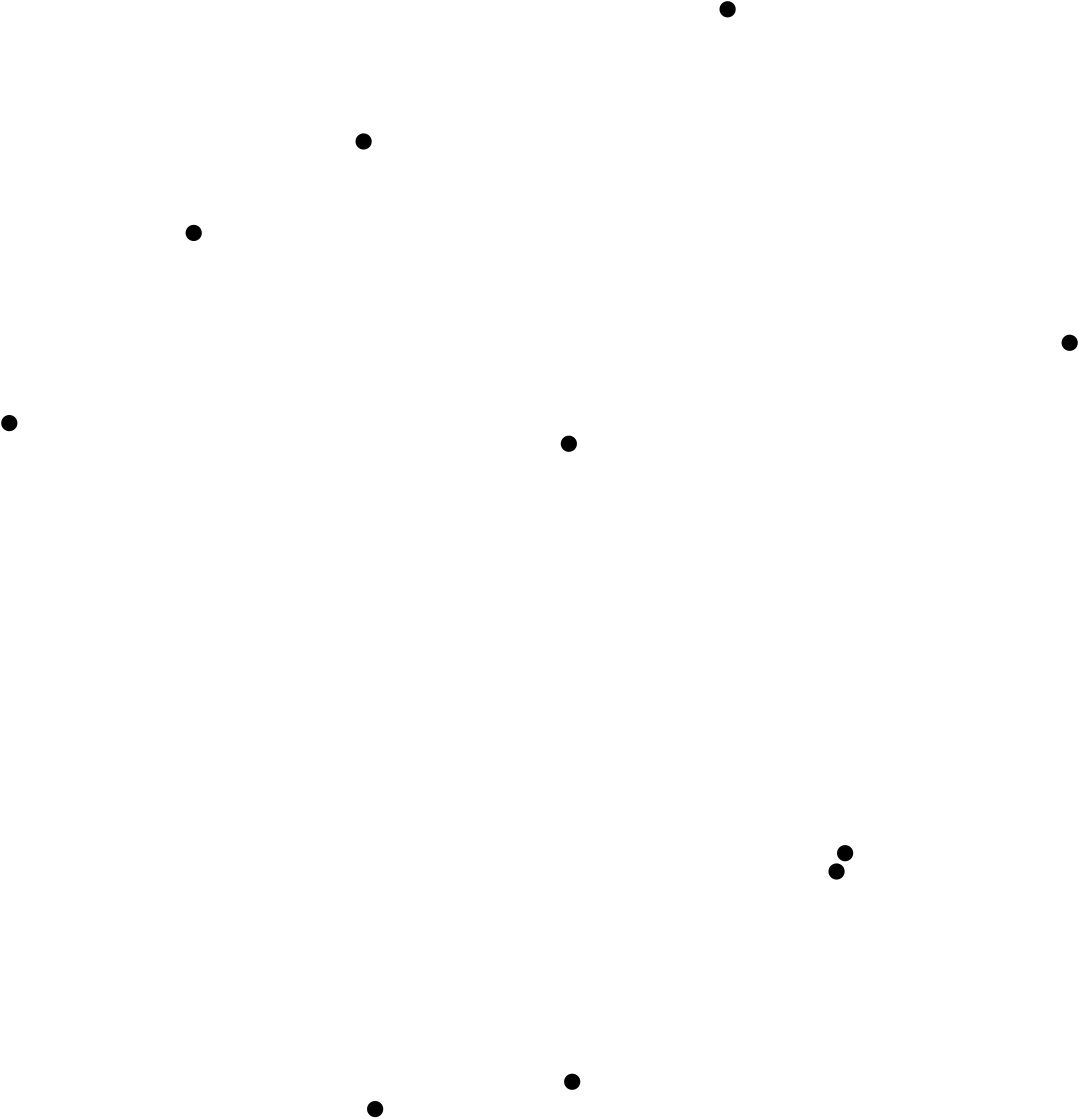
\includegraphics[width=\linewidth, frame]{10_81.png}
    \caption{Tipo de orden número 81 para $n=10$}
\end{figure}
\begin{figure}
    \centering
    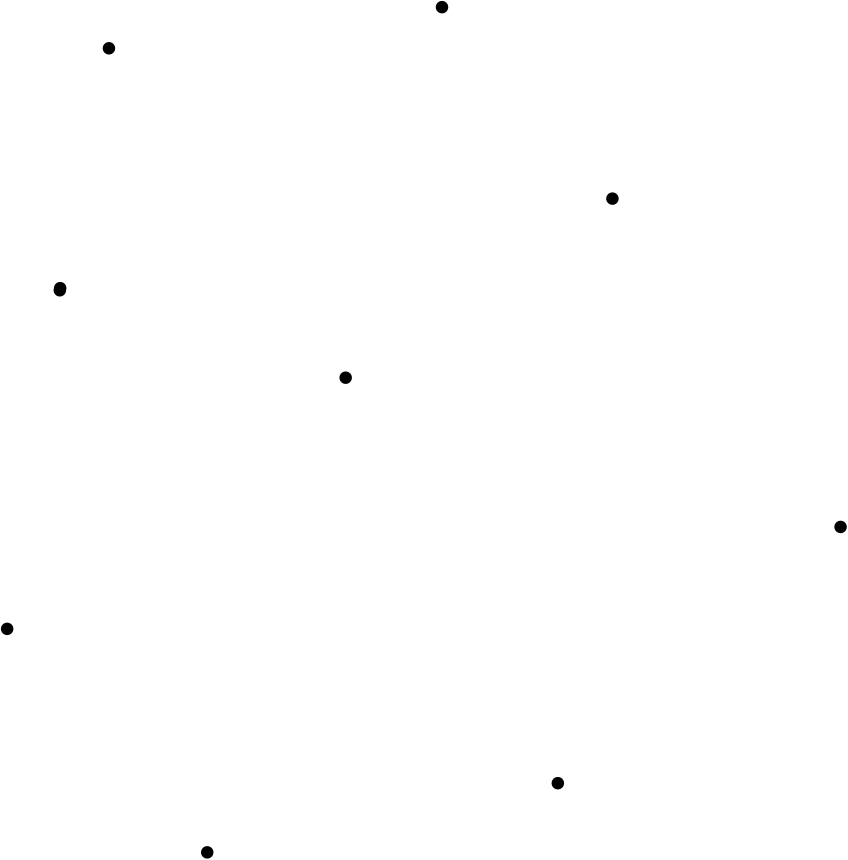
\includegraphics[width=\linewidth, frame]{10_1328.png}
    \caption{Tipo de orden número 1328 para $n=10$}
\end{figure}
\begin{figure}
    \centering
    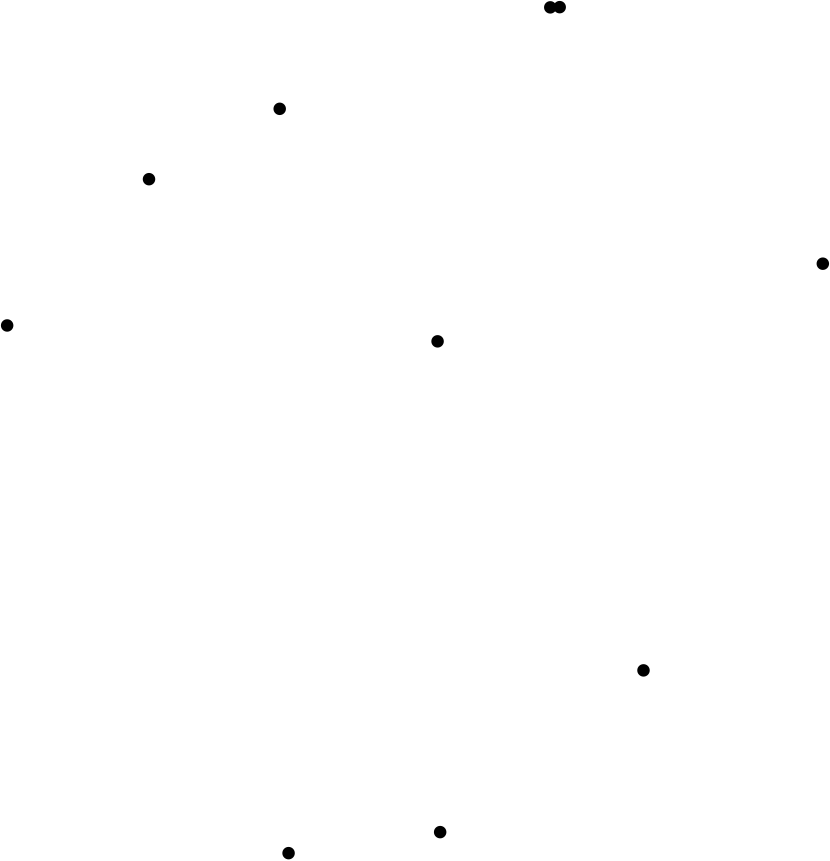
\includegraphics[width=\linewidth, frame]{10_2243.png}
    \caption{Tipo de orden número 2243 para $n=10$}
\end{figure}
